\documentclass{article}

\textwidth=6.5in
\textheight=8.5in
\voffset=-54pt
\oddsidemargin=0in
\evensidemargin=0in
\setlength{\parskip}{8pt}
\setlength{\parindent}{0pt}

\usepackage{amsmath, amssymb}
\usepackage{ifthen}

\usepackage[inline]{enumitem}
\setlist{topsep=0pt, parsep=8pt}

\usepackage[rgb,table]{xcolor}\convertcolorsUfalse
\usepackage{graphicx}

% change hyperref options
\PassOptionsToPackage{hyphens}{url}
\usepackage[bookmarks,colorlinks,linkcolor=black,citecolor=blue,pdfstartview=FitH,urlcolor=blue]{hyperref}
\hypersetup{pdfpagemode=UseNone}
\usepackage{bookmark}

\usepackage{graphicx}
\usepackage{multicol}
\usepackage{framed}
\usepackage{array}

\usepackage{icomma}

\usepackage{soul}
\usepackage[normalem]{ulem}

\usepackage{pgfplots}
\pgfplotsset{compat=1.18}  
\pgfplotscreateplotcyclelist{mycolor}{black, blue, red, green!70!black, magenta, purple, cyan, orange }  
\pgfplotsset{
  disabledatascaling,
  cycle list=tikzcolor, 
  axis lines=middle,
  every axis plot/.style={no marks, thick},
  every axis/.style={
    enlarge x limits=false,
    enlarge y limits=auto,
    xlabel style={at={(current axis.right of origin)},anchor=west},
    ylabel style={at={(current axis.above origin)},anchor=south},
    % extra x and y ticks for asymptotes
    extra x tick style={grid=major, grid style={dashed,black}},
    extra y tick style={grid=major, grid style={dashed,black}},
    /pgf/number format/1000 sep={},
  },    
  tick label style = {font=\footnotesize, fill=\currentbgcolor, inner sep=0pt},    
  xticklabel shift=1pt,    
  scaled ticks=false,
  scaled y ticks=false,
  unbounded coords=jump,
  samples=101,
  minor tick length=0,
  scatter/classes={
    open={mark=*,draw=black,fill=white, mark size=2, thin},
    closed={mark=*,draw=black,fill=black, mark size=2, thin}
  },
  width=3in,
}
\pgfplotsset{open/.style={only marks, mark=*, fill=white, thin, mark size=2}}
\pgfplotsset{closed/.style={only marks, mark=*, draw=black, fill=black,
    thin, mark size=2}}
\pgfplotsset{labeled/.style={nodes near coords, only marks, mark=*, draw=black, fill=black, thin, mark size=2, point meta=explicit symbolic}}

\usepackage{tikz}
\usetikzlibrary{
  matrix,%
  % enables the snake paths
  decorations.pathmorphing,%
  % enables bigger arrows
  decorations.markings,%
  decorations.pathreplacing,%
  decorations.text,%
  calc,%
  patterns,%
  shapes.geometric,%
  arrows,
  decorations.shapes,
  positioning,
  plotmarks,
  intersections
}
\tikzset{>=latex} % sets default arrow type in tikz
\tikzset{font=\normalsize}
\tikzset{mark size=1.5pt, mark options=thin}
\tikzset{pin distance=4pt,
  every pin edge/.style={<-, thin, shorten <= -2pt}}

\interfootnotelinepenalty=10000
\renewcommand{\thefootnote}{(\arabic{footnote})}

\usepackage{multirow, bigdelim}

% change to \usepackage[sols]{handout} to see solutions
\usepackage[]{handout}
\renewcommand{\workshopnote}{CA Notes.}    

\newcommand\iscurrentenumi[1]{%
  \ifthenelse{\equal{#1}{\theenumi}}{}{#1}}
\setenumerate[1]{ref=\#\arabic*}
\setenumerate[2]{ref=\protect\iscurrentenumi{\theenumi}(\alph*)}
\newcommand\enumiiprefix[2]{%
  \ifthenelse{{\equal{#1}{\theenumi}}\AND{\equal{#2}{(\alph{enumii})}}}{}{}%
  \ifthenelse{{\equal{#1}{\theenumi}}\AND{\NOT{\equal{#2}{(\alph{enumii})}}}}{#2}{}%
  \ifthenelse{\equal{#1}{\theenumi}}{}{#1#2}%
}
\setenumerate[3]{ref=\protect\enumiiprefix{\theenumi}{(\alph{enumii})}\roman*}

\makeatletter

% underline links               
\let\@href=\href
\renewcommand{\href}[2]{\@href{#1}{\ul{#2}}}

\makeatother

\definecolor{purple}{rgb}{0.5,0,1.0}

\newcommand{\doedfinity}[2][\newpage]{
  \begin{problem}[#1]
    Do the Edfinity assignment ``Problem Set #2''.

    We encourage you to write down any scratch work here, as well as
    things you want your future self to remember. Nothing you write
    here will be graded; it's just for you!
  \end{problem}
}

\newcommand{\psrnewpage}{\newpage}
\newcommand{\psreflection}[2][]{

  \ifthenelse{\not\equal{#1}{nocite}}{
    \begin{enumerate}[resume]
    \item
      \begin{problem}[1in]
        Please cite any help you got on this problem set:
        \begin{itemize}[nosep]
        \item If you worked with other students, please list their names here.
        \item If you used resources other than those on our Canvas site, please list them here.
        \end{itemize}
      \end{problem}

    \end{enumerate}
  }

  \probonly{%
    #2

    \psrnewpage

    \emph{Reflection space.} It's a good habit to take a few minutes at the end of each pset to reflect on what you learned and jot down notes to your future self. Here are a few reflection questions to get you started. Nothing you write here will be graded; it's just for you!
    \begin{itemize}
    \item Take a few minutes to look back at the problems. How could you explain to someone else how to do each problem? What was your strategy, and how did you know to use that strategy? If there are problems where you don't feel able to answer this, write down which ones they are. Come back to them in a few days when we post the homework solutions!

      \vspace{1.5in}

    \item Take a look back at the learning objectives on today's worksheet; how are you feeling about each one? If there are ones you know you need more practice with, write those down here.

      \vspace{1.5in}

    \item What did you find most challenging about this material? Do you have any lingering questions about it? If so, write them down here so you don't forget them. At some point, stop by office hours or MQC to ask!

      \vfill
    \end{itemize}      
  }
}

\usepackage{fancyhdr}
\lhead{\textcolor{white}{This content is protected and may not be shared, uploaded, or distributed.}}
\rhead{}
\rfoot{\vspace*{\fill}\footnotesize\textcopyright{} \emph{Harvard Math Ma}}
\renewcommand{\headrulewidth}{0pt}
\pagestyle{fancy}
\begin{document}

\begin{center}
  \large\textsc{Problem Set 20 - Maxima and Minima of Functions}
\end{center}

\begin{enumerate}
\item  \note{
    \begin{itemize}[nosep]
    \item (Follow-up from last time) Which functions are we able to differentiate using just the rules we've learned?
    \item (Follow-up from last time) When doing a tangent line approximation, how do you pick where to find the tangent line? 
    \item Identify local and global extrema on graph.
    \item Given $f$, $f'$, and $f''$ at a point, determine whether that point is a local min / local max /  neither / not enough info.
    \item Find critical points of a function (has one value where $f'$ is 0 and one value where $f'$ is undefined). 
    \end{itemize}
}

  \doedfinity{20}

\item    
  \begin{enumerate}
  \item Let $f(x) = |x^2 - 4|$.

    \begin{enumerate}
    \item

      \begin{grading}
        4 points:
        \begin{itemize}[nosep]
        \item 2 points for the graph:
          \begin{itemize}[nosep]
          \item If they do it using graph transformations: 0.5 for starting with a good graph of $x^2$, 0.5 for shifting down, 1 for doing the absolute value correctly
          \item If they plotted points, deduct 0.01 points (just so they know there's feedback) and give them feedback encouraging them to go to office hours / MQC to talk about a better way to do this
          \item If you can't tell how they got the graph, deduct 1 point for lacking an explanation. 
          \end{itemize}
        \item 0.5 for finding and labeling the $y$-intercept
        \item 1.5 for finding and labeling the $x$-intercepts
        \end{itemize}
      \end{grading}

      \begin{problem}[\stretch{5}]
        Without using technology, sketch a graph of $f$. Explain how you got it, and find and label all intercepts. 
      \end{problem}

      \begin{solution}
        We know that the graph of $y=x^2-4$ is the graph of $y=x^2$ shifted down 4 units. 
        The graph of $y=|x^2-4$ is graph of $y=x^2-4$, but will all of the sections
        below the $x$-axis reflected above the $x$-axis.
        The $y$-intercept is $f(0)=4$, and to find the $x$-intercepts, we can
        set $f(x)$ equal to zero and solve for $x$.
        \begin{align*}
          |x^2-4| &= 0 \\
          x^2 - 4 &= 0 \\
          x^2 &= 4 \\
          x &= \pm 2
        \end{align*}
        So the graph looks like this.
        \begin{center}
          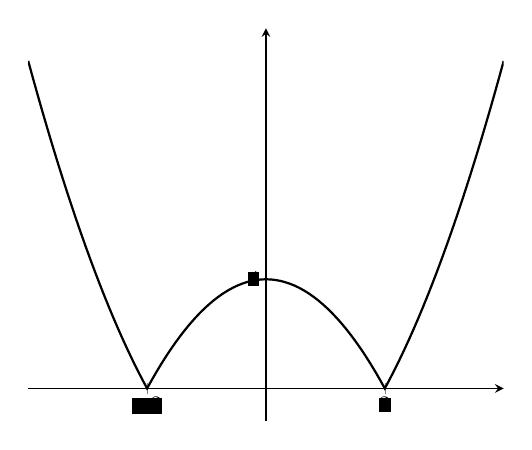
\begin{tikzpicture}
            \begin{axis}[ytick={4}, xtick={-2,2}]
              \addplot[domain=-4:4] {abs(x^2-4)};
            \end{axis}
          \end{tikzpicture}
        \end{center}
      \end{solution}

    \end{enumerate}
    Use the graph you sketched to answer the following questions. No explanation is needed.

    \begin{grading}
      1 point per question (6 points total)
    \end{grading}

    \begin{enumerate}[resume]
    \item
      \begin{problem}[\vfill]
        Where are the local minima of $f$? (Note: When we ask ``where'' maxima/minima occur, we're always asking for the $x$-values.) 
      \end{problem}

      \begin{solution}
        The local minima occur at $x=-2$ and $x=2$.
      \end{solution}

      \begin{problem}[\vfill]
        Where are the local maxima?
      \end{problem}

      \begin{solution}
        There is a local maximum at $x=0$. 
      \end{solution}

    \item
      \begin{problem}[\vfill]
        Does $f$ have a global maximum on $[-5, 3]$? If so, where? (In a question about where a global max/min happens, you should list \uline{all} of the $x$-values where the global max/min happens.) 
      \end{problem}

      \begin{solution}
        The global maximum on $[-5, 3]$ is at $x=-5$.
      \end{solution}

      \begin{problem}[\vfill]
        Does $f$ have a global minimum on $[-5, 3]$? If so, where?
      \end{problem}

      \begin{solution}
        The global minima on $[-5, 3]$ occur at $x=-2$ and $x=2$. 
      \end{solution}

    \item
      \begin{problem}[\vfill]
        Does $f$ have a global maximum on $(-5, 3)$? If so, where? 
      \end{problem}

      \begin{solution}
        $f$ does not have a global maximum on $(-5, 3)$.
      \end{solution}

      \begin{problem}[\vfill\newpage]
        Does $f$ have a global minimum on $(-5, 3)$? If so, where? 
      \end{problem}

      \begin{solution}
          The global minima on $(-5, 3)$ occur at $x=-2$ and $x=2$. 
      \end{solution}

    \end{enumerate}

  \item
    Let $f(x) = - \dfrac{1}{x} + 2$.

    \begin{enumerate}
    \item

      \begin{grading}
        4 points:
        \begin{itemize}[nosep]
        \item 1 point for the correct general shape
        \item 1 point for having shifted up so that the horizontal asymptote is at $y = 2$ (if they've shifted up but it isn't clear by how much, deduct 0.5)
        \item 1 point for finding and labeling the $x$-intercept
        \item 1 point for a reasonable explanation of how they got the graph. (If they plotted points here but not in (a), please give them the 0.01 deduction and feedback here.) 
        \end{itemize}
      \end{grading}

      \begin{problem}[\stretch{3}]
        Without using technology, sketch a graph of $f$. Explain how you got it, and label all asymptotes. Also find and label all intercepts. 
      \end{problem}

      \begin{solution}
        The parent graph is $y=\frac{1}{x}$. We take this graph, reflect it over the
        $x$-axis, and shift it up by 2 units. There is a vertical asymptote at $x=0$
        and a horizontal asymptote at $y=2$. There is no $y$-intercept.
        We can solve for the $x$-intercept.
        \begin{align*}
          -\frac{1}{x}+2 &= 0 \\
          2 &= \frac{1}{x} \\
          x &= \frac{1}{2}.
        \end{align*}
        The graph looks like this.
         \begin{center}
          \begin{tikzpicture}
            \begin{axis}[ytick=\empty, extra y ticks={2}, xtick={0.5}]
              \addplot[domain=-4:4] {-1/x + 2};
            \end{axis}
          \end{tikzpicture}
        \end{center}
      \end{solution}

    \end{enumerate}
    Use the graph you sketched to answer the following questions. No explanation is needed.

    \begin{grading}
      1 point per question (4 points total)
    \end{grading}

    \begin{enumerate}[resume]
    \item
      \begin{problem}[\vfill]
       Where are the local minima of $f$? 
      \end{problem}

      \begin{solution}
        $f$ has no local minima.
      \end{solution}

      \begin{problem}[\vfill]
        Where are the local maxima?
      \end{problem}

      \begin{solution}
        $f$ has no local maxima.
      \end{solution}

    \item
      \begin{problem}[\vfill]
        Does $f$ achieve a global maximum on $[1, \infty)$? If so, where? (Wording note: Asking if $f$ ``achieves'' or ``attains'' a global max/min is the same as asking if it ``has'' a global max/min. All 3 words are commonly used in this context.) 
      \end{problem}

      \begin{solution}
        $f$ does not attain a global maximum on $[1, \infty)$.
      \end{solution}

      \begin{problem}[\vfill\newpage]
        Does $f$ achieve a global minimum on $[1, \infty)$? If so, where?
      \end{problem}

      \begin{solution}
        On $[1, \infty)$, $f$ has a global minimum at $x=1$. 
      \end{solution}

    \end{enumerate}
  \end{enumerate}

\item \label{second-derivative-test-inconclusive-1}

  \note{This has a critical point where the Second Derivative Test is inconclusive.}

  Let $f(x) = x^5 - 5x^4$. 
  \begin{enumerate}
  \item \label{second-derivative-test-inconclusive-1-critical-numbers}

    \begin{grading}
      2.5 points: 0.5 for knowing to solve $f' = 0$, 0.5 for calculating $f'$ correctly, 1.5 for solving $f' = 0$ correctly.
    \end{grading}

    \begin{problem}[\stretch{0.5}]
      Find the critical points of $f(x)$.
    \end{problem}

    \begin{solution}
      The critical points are where $f'(x)$ is zero or undefined. Using the Power Rule,
      we can determine that $f'(x)=5x^4-20x^3$. This is never undefined. Solving
      $f'(x)=0$:
      \begin{align*}
        5x^4-20x^3 &= 0 \\
        5x^3(x-4) &= 0 \\
        x=0 \text{ or } x=4
      \end{align*}
      The critical points are $x=0$ and $x=4$.
    \end{solution}

  \item

    \begin{grading}
      2.5 points: 0.5 for calculating $f''$ correctly, 1 for analyzing each critical point correctly
    \end{grading}

    \begin{problem}[\vfill]
      What does the Second Derivative Test tell you about each critical point you found in \ref{second-derivative-test-inconclusive-1-critical-numbers}? (Tip: Factoring $f''(x)$ will make the computations easier.) 
    \end{problem}

    \begin{solution}
      First, we use the Power Rule to find that $f''(x)=20x^3-60x^2$. This can be rewritten
      as $f''(x)=20x^2(x-3)$. For the critical point $x=0$, $f''(0)=0$, so the Second
      Derivative Test is inconclusive. For the critical point $x=4$, $f''(4)=320$, so
      the Second Derivative Test tells us that there is a local minimum at $x=4$. 
    \end{solution}

  \item

    \begin{grading}
      2.5 points: 1.5 for making a correct sign chart, 1 for drawing correct conclusions from the sign chart
    \end{grading}

    \begin{problem}[\nstretch{1.25}]
      What does the First Derivative Test tell you about each critical point you found in \ref{second-derivative-test-inconclusive-1-critical-numbers}?
    \end{problem}

    \begin{solution}
      To carry out the First Derivative Test, we should make a sign chart for 
      $f'(x)=5x^3(x-4)$. We can determine the sign of $f'(x)$ on each interval
      by thinking about the graph of $f'(x)$ or by testing points.
      \begin{center}
        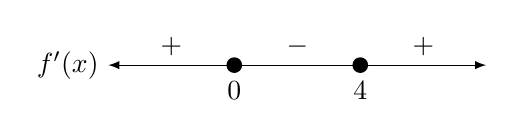
\begin{tikzpicture}[scale=0.8]
          \draw[<->] (-3,0) -- (3, 0);
          \node[left] at (-3,0) {$f'(x)$};
          \draw[shift={(-1,0)},color=black] (0pt,3pt) -- (0pt,-3pt) node[below] {$0$};
          \draw[shift={(1,0)},color=black] (0pt,3pt) -- (0pt,-3pt) node[below] {$4$};
          \node[circle, fill=black, inner sep=2pt] at (1,0) {};
          \node[circle, fill=black, inner sep=2pt] at (-1,0) {};
          \node[above] at (-2,0) {$+$};
          \node[above] at (0,0) {$-$};
          \node[above] at (2,0) {$+$};
        \end{tikzpicture}
      \end{center}
      Since $f'(x)$ changes from positive to negative at $x=0$, the First Derivative
      Test tells us that there is a local maximum at $x=0$. Since $f'(x)$ changes
      from negative to positive at $x=4$, the First Derivative Test tells us that
      there is a local minimum at $x=4$. 
    \end{solution}

  \item 

    \begin{grading}
      1 point. It's okay if they forget to mention the case where $f''(c)$ is undefined. 
    \end{grading}

    \begin{problem}[1.5in]
      \textbf{Reflect Back.} You just saw an example where the First Derivative Test gives more information than the Second Derivative Test. In what situations do you \uline{have} to use the First Derivative Test rather than the Second Derivative Test? Write a brief summary.
    \end{problem}

    \begin{solution} % Jason Bland
      We need to use the First Derivative Test instead of the Second Derivative Test for critical points $c$ where $f''(c)$ is either 0 or undefined. (In these cases, the Second Derivative Test gives no information.)
    \end{solution}

  \end{enumerate}

\item For each of the following functions, find all critical points, and classify each as a local maximum, local minimum, or neither. You get to decide whether to use the First Derivative Test or Second Derivative Test; please include a sentence saying which test you chose and why. Show your work in an organized way; make it easy for your reader to follow your reasoning. 

  \begin{enumerate}
  \item

    \begin{workshop}
      If students are having trouble deciding which test to use, encourage them to just try both. 
    \end{workshop}

    \begin{grading}
      5 points: 2 for finding the critical points, 2 for classifying them, 1 for explaining which test they chose and why. (They can use either the First Derivative Test or the Second Derivative Test.)
    \end{grading}

    \begin{problem}[\nstretch{1.5}]
      $f(x) = x^4 - x^2$
    \end{problem}

    \begin{solution}
      First, we find $f'(x)$. Using the Power Rule, $f'(x)=4x^3-2x$. The critical points
      are where $f'(x)$ is zero or undefined. It is never undefined. Solving $f'(x)=0$:
      \begin{align*}
        4x^3-2x &= 0 \\
        2x(2x^2-1) &= 0 \\
        x = 0 \text{ or } x = \pm \frac{1}{\sqrt{2}}.
      \end{align*}
      The critical points are $x=0$, $x=\pm\frac{1}{\sqrt{2}}$.

      To carry out the First Derivative Test, we create a sign chart.

      \begin{center}
        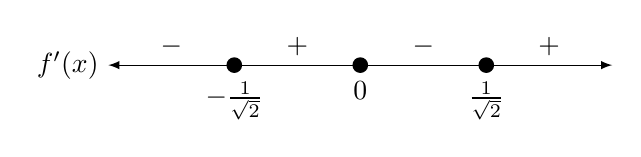
\begin{tikzpicture}[scale=0.8]
          \draw[<->] (-4,0) -- (4, 0);
          \node[left] at (-4,0) {$f'(x)$};
          \draw[shift={(0,0)},color=black] (0pt,3pt) -- (0pt,-3pt) node[below] {$0$};
          \draw[shift={(-2,0)},color=black] (0pt,3pt) -- (0pt,-3pt) node[below] 
          {$-\frac{1}{\sqrt{2}}$};
          \draw[shift={(2,0)},color=black] (0pt,3pt) -- (0pt,-3pt) node[below] 
          {$\frac{1}{\sqrt{2}}$};
          \node[circle, fill=black, inner sep=2pt] at (0,0) {};
          \node[circle, fill=black, inner sep=2pt] at (-2,0) {};
          \node[circle, fill=black, inner sep=2pt] at (2,0) {};
          \node[above] at (-3,0) {$-$};
          \node[above] at (-1,0) {$+$};
          \node[above] at (1,0) {$-$};
          \node[above] at (3,0) {$+$};
        \end{tikzpicture}
      \end{center}
      Since $f'(x)$ changes from negative to positive at $x=\pm \frac{1}{\sqrt{2}}$,
      there are relative minima at $x=\pm \frac{1}{\sqrt{2}}$. 
      Since $f'(x)$ changes from positive
      to negative at $x=0$, there is a relative maximum at $x=0$. 

      To conduct the Second Derivative Test, we would have to find $f''(x)$.
      Using the Power Rule again, $f''(x)=12x^2-2$. At $x=\pm \frac{1}{\sqrt{2}}$,
      $f''(\pm \frac{1}{\sqrt{2}}) = 4$. Since $f''(x)$ is positive at
      $x=\pm \frac{1}{\sqrt{2}}$, there are relative minima at $x=\pm \frac{1}{\sqrt{2}}$.
      At $x=0$, $f''(0)=-2$. Since $f''(x)$ is negative at $x=0$, there is a relative
      maximum at $x=0$.
    \end{solution}

  \item

    \begin{grading}
      2 points
    \end{grading}

    \begin{problem}[\vfill]
      $g(t) = t^3 + 3t + 1$
    \end{problem}

    \begin{solution}
      $g'(t)=3t^2+3=3(t^2+1)$, which is never 0 or undefined. So, there are \fbox{no critical points}.
    \end{solution}

  \end{enumerate}

\item \label{critical-points-reasoning-1}

  (Exploratory) Walter is trying to find the global maximum and minimum of a  function $f(x)$ that's continuous on $(-\infty, \infty)$. First, he finds that the critical points of $f(x)$ are $x = -2$, $1$, and $3$. Then, he figures out that $f'$ is negative on $(-\infty, -2)$, positive on $(-2, 1)$, negative on $(1, 3)$, and positive on $(3, \infty)$. He put this information together in the following chart:
  \begin{center}
    \begin{tikzpicture}
      \begin{axis}[axis y line=none, x axis line style={-}, xtick={-2, 1, 3}, ymin=-2, height=1in, width=3in]
        \addplot+[domain=-8.5:5., very thin]{0};
        \draw (axis cs: -8.5, -1.5) node[right] {sign of $f'$};
        \draw (axis cs: -3., -1.5) node{$-$};
        \draw (axis cs: -0.5, -1.5) node{$+$};
        \draw (axis cs: 2., -1.5) node{$-$};
        \draw (axis cs: 4., -1.5) node{$+$};
      \end{axis}
    \end{tikzpicture}
  \end{center}

  Answer each question below, with ``definitely yes'', ``definitely no'', or ``we don't have enough information''. Explain your reasoning; in addition, if we don't have enough information, sketch two different possibilities that show why.

  \begin{grading}
    2 points per part. Since it's exploratory, give full credit for a complete attempt (which should include an explanation or sketches). 
  \end{grading}

  \begin{enumerate}
  \item
    \begin{problem}[\vfill\newpage]
      Based on Walter's work so far, does $f(x)$ achieve a global
      minimum on $(-\infty, \infty)$?
    \end{problem}

    \begin{solution} 
      \fbox{Yes}; from the sign chart, we can see that $f(x)$ must have a global minimum at either $x = -2$ or $x = 3$. (Note that it's important that we were told that $f$ was continuous; if $f$ didn't have to be continuous, then it'd be possible for, say, $\displaystyle \lim_{x \to -2^+} f(x)$ to be $-\infty$, in which case $f$ wouldn't have a global minimum.)
    \end{solution}

  \end{enumerate}

  \begin{problemonly}
    Here's Walter's chart again:
    \begin{center}
      \begin{tikzpicture}
        \begin{axis}[axis y line=none, x axis line style={-}, xtick={-2, 1, 3}, ymin=-2, height=1in, width=3in]
          \addplot+[domain=-8.5:5., very thin]{0}; \draw (axis cs: -8.5, -1.5) node[right] {sign of $f'$}; \draw (axis cs: -3., -1.5) node{$-$}; \draw (axis cs: -0.5, -1.5) node{$+$}; \draw (axis cs: 2., -1.5) node{$-$}; \draw (axis cs: 4., -1.5) node{$+$};
        \end{axis}
      \end{tikzpicture}
    \end{center}
  \end{problemonly}

  \begin{enumerate}[resume]
  \item
    \begin{problem}[\vfill]
      Based on Walter's work so far, does $f(x)$ achieve a global maximum on $(-\infty, \infty)$? (Remember to explain and, if we don't have enough information, to sketch two different possibilities that show why.) 
    \end{problem}

    \begin{solution} 
      We \fbox{don't have enough information}. Here are two functions that both fit the sign chart; the first does not have a global maximum on $(-\infty, \infty)$ and the second does:
      \begin{center}
        \begin{tikzpicture}
          \begin{axis}[width=3in, xtick={-2, 1, 3}, ytick=\empty,
            height=2in]
            \addplot+[domain=-4.2:5.2]{15 + 6*x - (5*x^2)/2 - (2*x^3)/3 + x^4/4};
          \end{axis}
        \end{tikzpicture}
        \hspace{0.5in}
        {
          \makeatletter
          \pgfmathdeclarefunction{erf}{1}{%
            \begingroup
            \pgfmathparse{#1 > 0 ? 1 : -1}%
            \edef\sign{\pgfmathresult}%
            \pgfmathparse{abs(#1)}%
            \edef\x{\pgfmathresult}%
            \pgfmathparse{1/(1+0.3275911*\x)}%
            \edef\t{\pgfmathresult}%
            \pgfmathparse{%
              1 - (((((1.061405429*\t -1.453152027)*\t) + 1.421413741)*\t 
              -0.284496736)*\t + 0.254829592)*\t*exp(-(\x*\x))}%
            \edef\y{\pgfmathresult}%
            \pgfmathparse{(\sign)*\y}%
            \pgfmath@smuggleone\pgfmathresult%
            \endgroup
          }
          \makeatother   
          \begin{tikzpicture}
            \begin{axis}[width=3in, xtick={-2, 1, 3}, ytick=\empty,
              height=2in]
              \addplot+[domain=-8:8]{2/e^(x^2/4) + (4*x)/e^(x^2/4) - (2*x^2)/e^(x^2/4) + 2*sqrt(pi)*erf(x/2)};
            \end{axis}
          \end{tikzpicture}
        }
      \end{center}      
    \end{solution}

  \end{enumerate}

\item  \begin{grading}
    Nothing to grade here    
  \end{grading}

  \begin{problem}
    You should now be able to \href{https://www.gradescope.com/courses/873655}{see your graded exam in Gradescope}. There is good research showing that reflecting on your work is a very effective learning strategy, so please \href{https://www.youtube.com/watch?v=TOHCkI12mh0&t=43s}{look through the feedback} on your graded exam and fill out this \href{https://forms.gle/ffPRLMrMKszZ2Hzh8}{learning reflection survey}.
  \end{problem}

\end{enumerate}
\psreflection{For next class, read \href{https://canvas.harvard.edu/files/20608913/download?download_frd=1}{\S 4.2 of \emph{Calculus} by Hughes-Hallett et. al} through Example 1, or \href{https://activecalculus.org/single/sec-3-3-optimization.html}{Boelkins \S 3.3}.}
\end{document}
